\documentclass{article}

% 导入宏包
\usepackage{fancyhdr}
\usepackage{ctex}
\usepackage{listings}
\usepackage{graphicx}
\usepackage[a4paper, body={18cm,22cm}]{geometry}
\usepackage{amsmath,amssymb,amstext,wasysym,enumerate,graphicx}
\usepackage{float,abstract,booktabs,indentfirst,amsmath}
\usepackage{array}
\usepackage{multirow}
\usepackage{url}
\usepackage{diagbox}
\usepackage{enumitem}
\usepackage{xcolor}
\usepackage{makecell}
\usepackage{tikz}
\usetikzlibrary{positioning, arrows.meta}

% 设置段落
\renewcommand\arraystretch{1.4}
\setlength{\parindent}{2em}
\setCJKmonofont{黑体}

% 配置代码显示
\lstset{
	xleftmargin = 3em,
	xrightmargin = 3em,
	aboveskip = 1em,
	backgroundcolor = \color{white},
	basicstyle = \small\ttfamily,
	rulesepcolor = \color{gray},
	breaklines = true,
	numbers = left,
	numberstyle = \small,
	numbersep = -14pt,
	keywordstyle = \color{purple}\bfseries,
	commentstyle = \color{green!60!black}, % 修改注释颜色
	stringstyle = \color{red!60!green!90!blue!90},
	morekeywords = {ASSERT, int64_t, uint32_t},
	moreemph = {ASSERT, NULL},
	emphstyle = \color{red}\bfseries,
	moreemph = [2]{int64\_t, uint32\_t, tid\_t, uint8\_t, int16\_t, uint16\_t, int32\_t, size\_t, bool},
	emphstyle = [2]\color{purple}\bfseries,
	frame = shadowbox,
	showspaces = false,
	columns = fixed
	morecomment = [l][\color{green!60!black}]{+}, % 设置以+开头的代码行为绿色
}

%--------------------页眉--------------------%

\pagestyle{fancy}
\fancyhead[L]{}
\fancyhead[R]{}
\fancyhead[C]{华东师范大学软件工程学院实验报告}
\fancyfoot[C]{-\thepage-}
\renewcommand{\headrulewidth}{1.5pt}

%--------------------标题--------------------%

\begin{document}
	\begin{center}
		{\Large{\textbf{\heiti 华东师范大学软件工程学院实验报告}}}
		\begin{table}[htb]
			\flushleft
			\begin{tabular}{p{0.4\linewidth}p{0.27\linewidth}p{0.28\linewidth}}\\
				\textbf{实验课程}:操作系统实践  & \textbf{年级}:2023级       & \textbf{实验成绩}:  \\
				\textbf{实验名称}:Threads & \textbf{姓名}:顾翌炜         &                 \\
				\textbf{实验编号}:project-1     & \textbf{学号}:10235101527 & \textbf{实验日期}:2024/10/21  \\
				\textbf{指导教师}:陈闻杰     & \textbf{组号}:01            & \textbf{实验时间}:2024/10/21  \\ 
			\end{tabular}
		\end{table}
	\end{center}
	\rule{\textwidth}{2pt}
	
%--------------------正文--------------------%
%------------------实验目的------------------%
	\section{实验目的}
	
	试验一的最终任务就是在threads/中跑make check的时候, 27个test全pass。具体内容如下:
	\begin{enumerate}[noitemsep, label={{\arabic*})}]
		\item 修复现有的timer\_sleep()函数,消除忙等现象,提高系统效率。
		\item 实现一个基于优先级的线程调度系统,确保高优先级线程能够优先执行。
	\end{enumerate}
	\normalsize
	
	%------------------实验步骤------------------%
	\section{实验内容与实验步骤}
	
	首先cd到pintos/src/threads下,输入make check,测试结果得到:
	
    \begin{figure}[h]
    	\centering
    	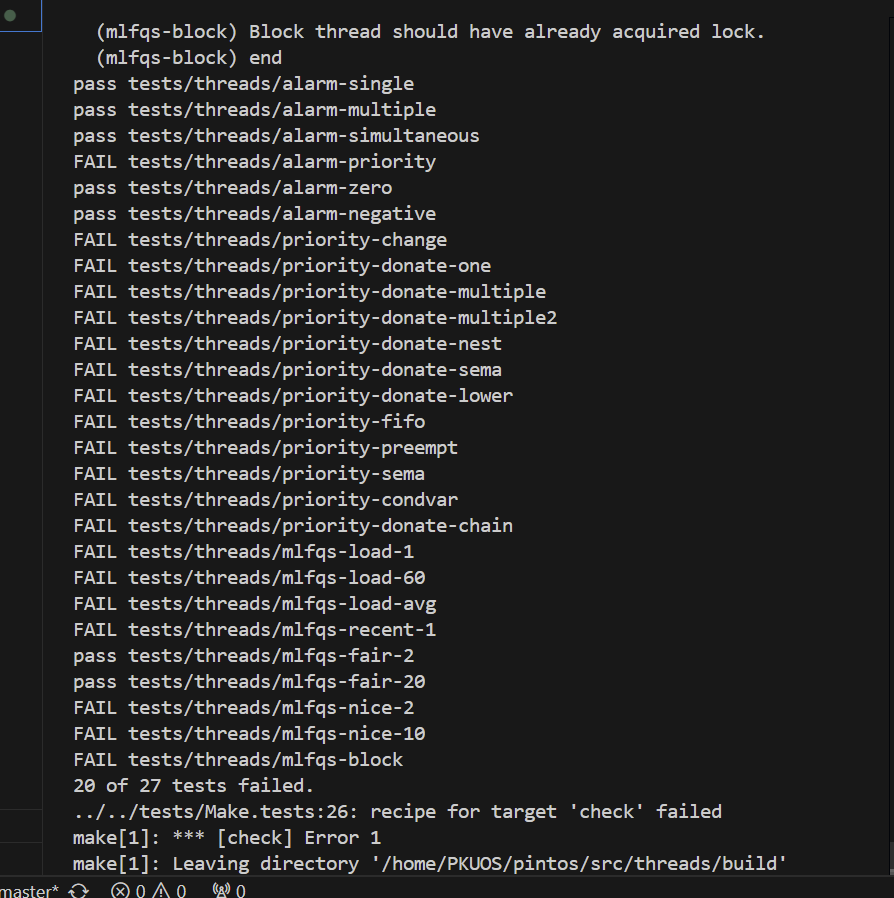
\includegraphics[width=8cm]{./img-project1/original.jpg}
    	\caption{make check before processing project1}
    	\label{fig:graph1}
    \end{figure}
    
    测试点在默认状态下通过了7/27个,接下来需要逐步修改完善代码,使本次实验需要的测试点全部通过。
	
	\subsection{Mission-1: 重新实现timer-sleep()函数}
	\subsubsection{分析原本的timer\_sleep()函数的实现思路}
	
	timer\_sleep函数位于\texttt{devices/timer.c}文件中。系统目前使用的是忙等实现方式,即线程不断地循环,直到时间片耗尽。需要更改timer\_sleep的实现方式。
	
	我们先来看一下位于devices目录下timer.c中的timer\_sleep实现:
	
	\begin{lstlisting}[xleftmargin = 4em,xrightmargin = 4em, aboveskip = 1em, numbers = left, language = C,title=原本的\texttt{timer\_sleep()}函数]
    /* Sleeps for approximately TICKS timer ticks.  
    Interrupts must be turned on. */
    void timer_sleep (int64_t ticks)
    {
    	int64_t start = timer_ticks ();
    	ASSERT (intr_get_level () == INTR_ON);
    	while (timer_elapsed (start) < ticks)
    	thread_yield();
    }
	\end{lstlisting}
	
	在这个函数中,调用了timer\_ticks函数,查找到这个函数:
	
	\begin{lstlisting}[xleftmargin = 4em,xrightmargin = 4em, aboveskip = 1em, numbers = left, language = C,title=\texttt{timer\_ticks()}函数]
    /* Returns the number of timer ticks since the OS booted. */
    int64_t timer_ticks (void)
    {
    	enum intr_level old_level = intr_disable ();
    	int64_t t = ticks;
    	intr_set_level (old_level);
    	return t;
    }
	\end{lstlisting}
	
	而在这个timer\_ticks中,intr\_level和intr\_disable也可以从代码中找到(此处略)
	
	intr\_level在代码中是一个结构体,代表能否被中断;而intr\_disable做了两件事情:1. 调用intr\_get\_level() 2. 直接执行汇编代码,调用汇编指令来保证这个线程不能被中断。
	
	\begin{lstlisting}[xleftmargin = 4em,xrightmargin = 4em, aboveskip = 1em, numbers = left, language = C,title=\texttt{get\_level()}函数]
    /* Returns the current interrupt status. */
    enum intr_level
    intr_get_level (void)
    {
    	uint32_t flags;
    	
    	/* Push the flags register on the processor stack, then pop the
    	value off the stack into `flags'.  See [IA32-v2b] "PUSHF"
    	and "POP" and [IA32-v3a] 5.8.1 "Masking Maskable Hardware
    	Interrupts". */
    	asm volatile ("pushfl; popl %0" : "=g" (flags));
    	
    	return flags & FLAG_IF ? INTR_ON : INTR_OFF;
    }
	\end{lstlisting}
	
	在这里,没有继续调用函数,所以 \texttt{intr\_disable()} 函数是调用的最远的地方了。
	
	综上所述:\texttt{timer\_ticks} 函数中的 \texttt{intr\_disable} 调用过程为:
	
	首先,\texttt{intr\_get\_level} 函数被用来获取当前的中断级别。随后,\texttt{intr\_disable} 执行两个关键步骤:一是将中断级别设置为禁止中断,二是返回之前的中断级别。这样,我们就可以理解在 \texttt{timer\_ticks} 函数的第4行,实际上是在执行一个保护操作:确保在获取计时器期间不会被中断,并在操作完成后恢复之前的中断状态,这一过程的中间状态被存储在 \texttt{timer\_ticks()} 这个函数中的变量 \texttt{old\_level} 中。\\[1em]
	
	再回到刚刚在看的 \texttt{timer\_ticks()},其函数的剩余操作包括:使用局部变量 \texttt{t} 获取全局变量 \texttt{ticks} 的值。此外,还调用了 \texttt{intr\_set\_level} 函数以恢复之前的中断状态。
	
	\begin{lstlisting}[xleftmargin = 4em,xrightmargin = 4em, aboveskip = 1em, numbers = left, language = C,title=\texttt{set\_level()}函数]
    /* Enables or disables interrupts as specified by LEVEL and
    returns the previous interrupt status. */
    enum intr_level
    intr_set_level (enum intr_level level)
    {
    	return level == INTR_ON ? intr_enable () : intr_disable ();
    }
	\end{lstlisting}
	
	再来观察 \texttt{intr\_enable} 和 \texttt{intr\_context} 函数,可以知道:如果之前是允许中断的(INTR\_ON)则enable,否则就disable。那么我们可以得到:timer\_ticks这个函数的完整作用:
	
	获取 \texttt{ticks} 的当前值并返回。第4行和第6行的作用是确保这一过程不会被中断。
	
	从$"static$ $int64\_t$ $ticks;"$可以知道:从pintos被启动开始, ticks就一直在计时, 代表着操作系统执行单位时间的前进计量。
	
	\begin{lstlisting}[xleftmargin = 4em,xrightmargin = 4em, aboveskip = 1em, numbers = left, language = C,title=\texttt{timer\_sleep()}函数中的部分代码]
    while (timer_elapsed (start) < ticks)
        thread_yield();
	\end{lstlisting}
	
	\texttt{timer\_sleep} 函数执行时,\texttt{start} 获取起始时间。函数断言必须可以被中断,否则会一直死循环。之后,函数进入循环。
	
	在timer\_sleep这个函数中的ticks作为形参,并不是全局变量,所以观察一下timer\_elapsed()函数。阅读发现:\texttt{timer\_elapsed} 返回了当前时间距离 \texttt{then} 的时间间隔。因此,这个循环实质上是在 \texttt{ticks} 时间内不断执行 \texttt{thread\_yield}。\\[1em]
	
	最后来看thread\_yield()这个函数:
		
	\begin{lstlisting}[xleftmargin = 4em,xrightmargin = 4em, aboveskip = 1em, numbers = left, language = C,title=\texttt{thread\_yield()}函数]
    /* Yields the CPU.  The current thread is not put to sleep and
    may be scheduled again immediately at the scheduler's whim. */
    void thread_yield (void)
    {
    	struct thread *cur = thread_current ();
    	enum intr_level old_level;
    	
    	ASSERT (!intr_context ());
    	
    	old_level = intr_disable ();
    	if (cur != idle_thread)
    	list_push_back (&ready_list, &cur->elem);
    	cur->status = THREAD_READY;
    	schedule ();
    	intr_set_level (old_level);
    }
	\end{lstlisting}
	
	在这个函数的第5行中,用到了 \texttt{thread\_current()} 函数,其实无需再去阅读具体代码,由其函数名称就可以看出:这个函数的作用就是返回当前线程起始指针。
	
	继续来看 \texttt{thread\_yield()} 函数,第8行的 \texttt{ASSERT} 是一个软中断。后面的if判断语句就是,若当前的线程不是空闲的,那么就调用 \texttt{list\_push\_back} 来将当前的线程放到就绪队列里,并把线程改成THREAD\_READY状态。再调用的 \texttt{schedule()} 函数,\texttt{schedule()} 其实就是拿下一个线程切换过来继续run。
	
	所以总结来说,\texttt{thread\_yield()} 其实就是把当前线程扔到就绪队列里,然后重新 \texttt{schedule()}。\\[1em]
	
	分析到此,\texttt{timer\_sleep} 就是在ticks时间内,如果线程处于running状态就不断把他扔到就绪队列不让他执行。所以它的缺点也就很显而易见了:
	
	线程依然不断在cpu就绪队列和running队列之间来回,占用了cpu资源。所以我的想法是:用一种唤醒机制来实现这个函数,使得线程在休眠的时候不会占用CPU资源。
	
	\subsubsection{重新实现timer\_sleep()函数}
	
	\textbf{实现思路:} 当调用timer\_sleep()函数时,我们会使线程进入阻塞状态,并在线程的数据结构中新增一个成员sleep\_ticks,用以追踪线程被暂停的具体时长。接着,我们利用操作系统的时钟中断机制(每次tick都会触发一次),来检查线程的状态。在每次检查过程中,我们会将sleep\_ticks的值减1。一旦该值降至0,即表示线程的等待时间已满,此时将解除线程的阻塞状态,使其恢复运行。
	
	\textbf{具体代码:}
	
	\begin{lstlisting}[xleftmargin = 4em,xrightmargin = 4em, aboveskip = 1em, numbers = left, language = C,title=修改后的 \texttt{timer\_sleep()}函数]
    /* Sleeps for approximately TICKS timer ticks.  Interrupts must
    be turned on. */
    void timer_sleep (int64_t ticks)
    {
    	if (ticks <= 0)
    	{
    	    return;  // 当ticks小于0的时候,等待时间已满,直接返回
    	}
    	ASSERT (intr_get_level () == INTR_ON);
    	
    	enum intr_level old_level = intr_disable ();  // 关闭中断
    	struct thread *current_thread = thread_current ();
    	current_thread->sleep_ticks = ticks;  // 设置sleep_ticks
    	thread_block ();  // 阻塞当前线程
    	intr_set_level (old_level);  // 恢复中断
    }
	\end{lstlisting}
	
	\texttt{timer\_sleep()} 函数中的 \texttt{intr\_disable()}、 \texttt{thread\_current} 等函数的实现无需改变,直接使用原有的函数逻辑即可。
	
	接下来在Thread的结构体中加上sleep\_ticks成员:int64\_t sleep\_ticks;
	
	\begin{lstlisting}[xleftmargin = 4em,xrightmargin = 4em, aboveskip = 1em, numbers = left, language = C, title=修改后的线程结构体]
    struct thread
    {
        /* Owned by thread.c. */
        tid_t tid;                    /* Thread identifier. */
        enum thread_status status;    /* Thread state. */
        char name[16];                /* Name (for debugging purposes). */
        uint8_t *stack;               /* Saved stack pointer. */
        int priority;                 /* Priority. */
        struct list_elem allelem;     /* List element for all threads list. */
        	
        /* Shared between thread.c and synch.c. */
        struct list_elem elem;        /* List element. */
        
        /* 新增的成员-被暂停的具体时长 */
        int64_t sleep_ticks;          /* Sleep ticks. */
        	
        #ifdef USERPROG
        /* Owned by userprog/process.c. */
        uint32_t *pagedir;            /* Page directory. */
        #endif
        	
        /* Owned by thread.c. */
        unsigned magic;               /* Detects stack overflow. */
    };
	\end{lstlisting}
	
	接下来就需要在函数中初始化这个sleep\_ticks变量,此处在thread\_create()函数中,将sleep\_ticks初始化为0。(下面函数中的第20行)
	
	\begin{lstlisting}[xleftmargin = 4em,xrightmargin = 4em, aboveskip = 1em, numbers = left, language = C, title=修改后的\texttt{thread\_create()}函数]
    tid_t thread_create (const char *name, int priority,
    thread_func *function, void *aux) 
    {
    	struct thread *t;
    	struct kernel_thread_frame *kf;
    	struct switch_entry_frame *ef;
    	struct switch_threads_frame *sf;
    	tid_t tid;
    	
    	ASSERT (function != NULL);
    	
    	/* Allocate thread. */
    	t = palloc_get_page (PAL_ZERO);
    	if (t == NULL)
    	    return TID_ERROR;
    	
    	/* Initialize thread. */
    	init_thread (t, name, priority);
    	tid = t->tid = allocate_tid ();
    	t->sleep_ticks = 0; // 初始化 sleep_ticks 为 0
    	
    	/* Stack frame for kernel_thread(). */
    	kf = alloc_frame (t, sizeof *kf);
    	kf->eip = NULL;
    	kf->function = function;
    	kf->aux = aux;
    	
    	/* Stack frame for switch_entry(). */
    	ef = alloc_frame (t, sizeof *ef);
    	ef->eip = (void (*) (void)) kernel_thread;
    	
    	/* Stack frame for switch_threads(). */
    	sf = alloc_frame (t, sizeof *sf);
    	sf->eip = switch_entry;
    	sf->ebp = 0;
    	
    	/* Add to run queue. */
    	thread_unblock (t);
    	
    	return tid;
    }
	\end{lstlisting}
	
	由于我们的 \texttt{sleep\_ticks} 是在每次检查过程中,将其值减1直至0时,解除线程的阻塞状态,使其恢复运行。所以需要在调用它的 \texttt{timer\_sleep()} 函数中,将当前线程的 \texttt{sleep\_ticks} 设置为其需要等待的时长。(参见前面的代码)\\[1em]
	
	最后一步,修改 \texttt{timer\_interrupt()} 函数,从而实现对于 \texttt{sleep\_ticks} 的更新,具体步骤如下:
	
	1. 使用使用thread\_foreach() 函数,遍历所有线程,将sleep\_ticks 减1
	
	2. 如果sleep\_ticks 为0,则将线程唤醒
	
	\begin{lstlisting}[xleftmargin = 4em,xrightmargin = 4em, aboveskip = 1em, numbers = left, language = C, title=修改后的\texttt{timer\_interrupt()}函数]
    /* Timer interrupt handler. */
    static void
    timer_interrupt (struct intr_frame *args UNUSED)
    {
    	ticks++;
    	thread_tick ();
    	thread_foreach (thread_tick_sleep, NULL); // 每次中断都调用 
    }
	\end{lstlisting}
	
	在这个函数中,有 \texttt{thread\_tick\_sleep} 和 \texttt{thread\_foreach} 这两个函数,具体如下:
	
	\begin{lstlisting}[xleftmargin = 4em,xrightmargin = 4em, aboveskip = 1em, numbers = left, language = C, title=\texttt{thread\_foreach()}函数]
    /* Invoke function 'func' on all threads, passing along 'aux'.
    This function must be called with interrupts off. */
    void thread_foreach (thread_action_func *func, void *aux)
    {
    	struct list_elem *e;
    	
    	ASSERT (intr_get_level () == INTR_OFF);
    	
    	for (e=list_begin(&all_list); e!=list_end(&all_list); e=list_next(e))
    	{  // 遍历list里所有的线程
            struct thread *t = list_entry (e, struct thread, allelem);
            func (t, aux);  // 对每个线程执行func函数
    	}
    }
	\end{lstlisting}
	
	所以我需要实现一下 \texttt{thread\_tick\_sleep} 函数。
	
	首先在thread.h文件中声明 \texttt{thread\_tick\_sleep} 函数,然后在thread.c文件中进行编写。
	
	\begin{lstlisting}[xleftmargin = 4em,xrightmargin = 4em, aboveskip = 1em, numbers = left, language = C, title=\texttt{thread\_tick\_sleep()}函数]
    void thread_tick_sleep (struct thread *t, void *aux UNUSED)
    {
    	if (t->status==THREAD_BLOCKED && t->sleep_ticks>0) // 如果休眠时间大于0
    	{
            t->sleep_ticks--; // 休眠时间减一
            if (t->sleep_ticks == 0) // 如果休眠时间到了
            {
                thread_unblock (t); // 唤醒
            }
    	}
    }
	\end{lstlisting}
	
	这样timer\_sleep函数唤醒机制就实现了。
	
	\subsection{Mission-2: 基于优先级的线程调度}
	
	接下来继续解决第二个任务:实现一个基于优先级的线程调度系统,确保高优先级线程能够优先执行。
	
	首先观察Thread这个结构体(具体代码在Mission-1中有展示),发现这个结构体里本身就有一个priority,所以我们后续只需要对每个线程的已有的priority进行比较就可以得到我们想要的结果。并且对于priority也有一定的约束条件,具体如下:
	
	\begin{lstlisting}[xleftmargin = 4em,xrightmargin = 4em, aboveskip = 1em, numbers = left, language = C, title=\texttt{priority}约束]
    /* Thread priorities. */
    #define PRI_MIN 0                       /* Lowest priority. */
    #define PRI_DEFAULT 31                  /* Default priority. */
    #define PRI_MAX 63                      /* Highest priority. */
	\end{lstlisting}
	
	利用之前对 \texttt{timer\_sleep()} 函数的分析,我们可以知道,这个Mission中对于优先级调度的实现的核心思想是:让就绪队列是一个优先级队列(Priority scheduling),那么我们在实现这一目标的时候可以理解为:每次往队列中插入新的线程的时候,是按照优先级来插入的,这样一来就能保证我们的队列是一个优先级队列。
	
	结合代码,我们可以发现,涉及到将线程插入到就绪队列的函数总共有以下三个:
	
	~~~~1. \texttt{thread\_unblock}
	
	~~~~2. \texttt{init\_thread}
	
	~~~~3. \texttt{thread\_yield}
	
	\subsubsection{依次修改三个有关插入线程的函数,通过测试 \texttt{alarm\_priority} }
	
	由刚刚的分析可以得出:只需要在上面三个函数中保持就绪队列是一个优先级队列即可。那接下来就按照顺序来依次分析。
	
	首先来看 \texttt{thread\_unblock} ,这里面的插入线程的代码是: \texttt{list\_push\_back (\&ready\_list, \&t->elem);},这个的意思是直接将线程放在了队列的尾部,也就是一个先进先出的FIFO逻辑,因为每次取出Thread都是取出头部,所以我们需要修改一下插入的位置。
	
	阅读 \texttt{/lib/kernel/} ,研究pintos里队列的实现:
	
	\begin{lstlisting}[xleftmargin = 4em,xrightmargin = 4em, aboveskip = 1em, numbers = left, language = C, title=\texttt{pintos}里的list]
    /* List element. */
    struct list_elem
    {
    	struct list_elem *prev;     /* Previous list element. */
    	struct list_elem *next;     /* Next list element. */
    };
    
    /* List. */
    struct list
    {
    	struct list_elem head;      /* List head. */
    	struct list_elem tail;      /* List tail. */
    };
	\end{lstlisting}
	
	这个list的实现是一个常见的队列这个数据结构。通过继续翻阅代码,找到了一个叫做 \texttt{list\_insert\_ordered} 的函数,根据函数名就可以知道这是用来给list排序的函数,那么我们可以断定,需要修改的就是这个函数了。
	
	\begin{lstlisting}[xleftmargin = 4em,xrightmargin = 4em, aboveskip = 1em, numbers = left, language = C, title=\texttt{list\_insert\_ordered}函数]
    /* Inserts ELEM in the proper position in LIST, which must be
    sorted according to LESS given auxiliary data AUX.
    Runs in O(n) average case in the number of elements in LIST. */
    void list_insert_ordered (struct list *list, struct list_elem *elem, list_less_func *less, void *aux)
    {
    	struct list_elem *e;
    	
    	ASSERT (list != NULL);
    	ASSERT (elem != NULL);
    	ASSERT (less != NULL);
    	
    	for (e = list_begin (list); e != list_end (list); e = list_next (e))
    	if (less (elem, e, aux))
    	    break;
    	return list_insert (e, elem);
    }
	\end{lstlisting}
	
	所以回到一开始看的那个 \texttt{thread\_unblock} 函数,把 \texttt{list\_push\_back} 改成: \texttt{list\_insert\_ordered\\ (\&ready\_list, \&t->elem, (list\_less\_func *) \&thread\_cmp\_priority, NULL);}
	
	然后需要实现的是其中的 \texttt{thread\_cmp\_priority} 函数,具体如下:
	
	\begin{lstlisting}[xleftmargin = 4em,xrightmargin = 4em, aboveskip = 1em, numbers = left, language = C, title=\texttt{thread\_cmp\_priority}函数]
    /* priority compare function. */
    bool thread_cmp_priority (const struct list_elem *a, const struct list_elem *b, void *aux UNUSED)
    {
    	return list_entry(a, struct thread, elem)->priority > list_entry(b, struct thread, elem)->priority;
    }
	\end{lstlisting}
	
	同理,对 \texttt{thread\_yield} 和 \texttt{thread\_init} 里的 \texttt{list\_push\_back} 作同样的修改(修改后的代码略)。在进行了这些修改以后,\texttt{alarm\_priority} 这个测试点pass了。
	
	\subsubsection{通过测试 \texttt{alarm-priority, priority-change, priority-fifo} 和 \texttt{priority-preempt}}
	
	抢占式调度的测试其实就是:在创建一个线程的时候,如果线程高于当前线程就先执行创建的线程。
	
	\begin{lstlisting}[language=Python, caption={Priority Change Example}]
    Acceptable output:(priority-change) begin
        (priority-change) Creating a high-priority thread 2.
        (priority-change) Thread 2 now lowering priority.
        (priority-change) Thread 2 should have just lowered its priority.
        (priority-change) Thread 2 exiting.
        (priority-change) Thread 2 should have just exited.
        (priority-change) end
    Differences in 'diff-u' format:
        (priority-change) begin
        (priority-change) Creating a high-priority thread 2.
        (priority-change) Thread 2 now lowering priority.
        (priority-change) Thread 2 should have just lowered its priority.
        (priority-change) Thread 2 exiting.
        (priority-change) Thread 2 should have just exited.
        (priority-change) end
	\end{lstlisting}
	
	因此,我们可以总结如下:
	
	在测试中,我们创建了一个名为thread1的线程,它生成了一个内核线程thread2,其优先级设置为\\PRI\_DEFAULT+1。由于thread2具有较高的优先级,系统立即将执行权交给了thread2,导致thread1进入阻塞状态。在thread2执行期间,它调用了changing\_thread函数,将自己的优先级调整为PRI\_DEFAULT-1,这样一来,thread1的优先级就相对更高了。
	
    当thread2在最后一个消息输出处被阻塞时,控制权转交给了thread1。随后,thread1将自己的优先级进一步降低到PRI\_DEFAULT-2,使得thread2的优先级再次高于thread1。于是,执行权又回到了thread2,它继续执行并输出thread1的消息。这一系列的优先级调整和线程切换,最终产生了图中所示的测试输出结果。
    
    所以我们可以知道:在设置一个线程优先级要立即重新考虑所有线程执行顺序, 重新安排执行顺序。所以直接在线程设置优先级的时候调用thread\_yield即可,相当于把当前线程重新丢到就绪队列中继续执行, 保证了执行顺序。(当然,如果在创建线程的时候, 如果新创建的线程比主线程优先级高的话也要调用thread\_yield)
	
	\begin{lstlisting}[xleftmargin = 4em,xrightmargin = 4em, aboveskip = 1em, numbers = left, language = C, title=\texttt{thread\_set\_priority}函数]
    /* Sets the current thread's priority to NEW_PRIORITY. */
    void thread_set_priority (int new_priority)
    {
    	thread_current ()->priority = new_priority;
    	thread_yield ();
    }
	\end{lstlisting}
	
	接下来,我们需要修改 \texttt{thread\_create()} 函数,使得线程在创建的时候,按照优先级的顺序插入就绪队列。在函数的最后把创建的线程unblock了之后加上和主线程的优先级的比较函数:
	
	\begin{lstlisting}[xleftmargin = 4em,xrightmargin = 4em, aboveskip = 1em, numbers = left, language = C, title=\texttt{thread\_create}函数结尾补充:]
    if (thread_current ()->priority < priority)
    {
        thread_yield ();
    }
	\end{lstlisting}
	
	完整的 \texttt{thread\_create()} 函数如下所示:
	
	\begin{lstlisting}[xleftmargin = 4em,xrightmargin = 3em, aboveskip = 1em, numbers = left, language = C, title=修改后的\texttt{thread\_create()}函数]
    tid_t
    thread_create (const char *name, int priority,
    thread_func *function, void *aux) 
    {
    	struct thread *t;
    	struct kernel_thread_frame *kf;
    	struct switch_entry_frame *ef;
    	struct switch_threads_frame *sf;
    	tid_t tid;
    	
    	ASSERT (function != NULL);
    	
    	/* Allocate thread. */
    	t = palloc_get_page (PAL_ZERO);
    	if (t == NULL)
    	return TID_ERROR;
    	
    	/* Initialize thread. */
    	init_thread (t, name, priority);
    	tid = t->tid = allocate_tid ();
    	t->sleep_ticks = 0;
    	
    	/* Stack frame for kernel_thread(). */
    	kf = alloc_frame (t, sizeof *kf);
    	kf->eip = NULL;
    	kf->function = function;
    	kf->aux = aux;
    	
    	/* Stack frame for switch_entry(). */
    	ef = alloc_frame (t, sizeof *ef);
    	ef->eip = (void (*) (void)) kernel_thread;
    	
    	/* Stack frame for switch_threads(). */
    	sf = alloc_frame (t, sizeof *sf);
    	sf->eip = switch_entry;
    	sf->ebp = 0;
    	
    	/* Add to run queue. */
    	thread_unblock (t);
    	
    	/* 优先级调度 */
    	if (thread_current ()->priority < priority)
    	{
    		thread_yield ();
    	}
    	
    	return tid;
    }
	\end{lstlisting}
	
	这样,我们就可以通过测试 \texttt{alarm-priority, priority-change, priority-fifo} 和 \texttt{priority-preempt}了。
	
	\subsubsection{通过测试 \texttt{priority-priority-*} }
	
	接下来需要实现的是优先级捐赠。同理先阅读测试文件,分析需要进行哪些修改。
	
	先来关注priority-donate-one的测试代码:
	
	\begin{lstlisting}[xleftmargin = 4em,xrightmargin = 4em, aboveskip = 1em, numbers = left, language = C, title=\texttt{thread\_create}函数结尾补充:]
    void test_priority_donate_one (void)
    {
    	struct lock lock;
    	
    	/* This test does not work with the MLFQS. */
    	ASSERT (!thread_mlfqs);
    	
    	/* Make sure our priority is the default. */
    	ASSERT (thread_get_priority () == PRI_DEFAULT);
    	
    	lock_init (&lock);
    	lock_acquire (&lock);
    	thread_create ("acquire1", PRI_DEFAULT + 1, acquire1_thread_func, &lock);
    	msg ("This thread should have priority %d.  Actual priority: %d.",
    	    PRI_DEFAULT + 1, thread_get_priority ());
    	thread_create ("acquire2", PRI_DEFAULT + 2, acquire2_thread_func, &lock);
    	msg ("This thread should have priority %d.  Actual priority: %d.",
    	    PRI_DEFAULT + 2, thread_get_priority ());
    	lock_release (&lock);
    	msg ("acquire2, acquire1 must already have finished, in that order.");
    	msg ("This should be the last line before finishing this test.");
    }
    
    static void acquire1_thread_func (void *lock_)
    {
    	struct lock *lock = lock_;
    	
    	lock_acquire (lock);
    	msg ("acquire1: got the lock");
    	lock_release (lock);
    	msg ("acquire1: done");
    }
    
    static void acquire2_thread_func (void *lock_)
    {
    	struct lock *lock = lock_;
    	
    	lock_acquire (lock);
    	msg ("acquire2: got the lock");
    	lock_release (lock);
    	msg ("acquire2: done");
    }
	\end{lstlisting}
	
	分析过程如下:最初主线程主动获取了一个lock(第11行),它的优先级被设定为PRI\_DEFAULT。随后,我们在第13和第16行主动给创建了两个优先级更高的新的线程,名为 \texttt{acquire1} 和 \texttt{acquire2} ,即 \texttt{PRI\_DEFAULT+1} 和 \texttt{PRI\_DEFAULT+2},这两个线程被设计为在获取锁时被阻塞。
	
	而后在第19行,主线程通过 \texttt{lock\_release} 主动释放锁,但是由于这时两个新线程的优先级高于主线程,它们会优先尝试获取锁(由于 \texttt{acquire2} 的优先级更高,它首先获取了锁, \texttt{acquire1} 在 \texttt{acquire2} 线程之后获取了锁)。
	
	再通过msg打印测试结果,确认 \texttt{acquire2} 线程先完成,然后再是 \texttt{acquire1} 。
	
	简而言之,这项测试旨在确认当一个线程释放锁时,它是否能够正确地将优先级传递给正在等待该锁的其他线程,以确保线程按照优先级来顺序获取锁。\\[1em]
	
	为了通过这个测试,首先,我们需要修改 \texttt{lock\_acquire()} 函数,使得线程在获取锁的时候,如果锁已经被占用,且当前线程的优先级大于锁的持有者的优先级,则将当前线程的优先级赋值给锁的持有者。
	
	\begin{lstlisting}[language=C, title=修改后的\texttt{lock\_acquire()}函数]
    void lock_acquire (struct lock *lock)
    {
    	ASSERT (lock != NULL);
    	ASSERT (!intr_context ());
    	ASSERT (!lock_held_by_current_thread (lock));
    	
    	if (lock->holder != NULL && lock->holder->priority < thread_current ()->priority)
    	{
    		lock->holder->priority = thread_current ()->priority;
    	}
    	
    	sema_down (&lock->semaphore);
    	lock->holder = thread_current ();
    }
	\end{lstlisting}
	
	接下来修改 \texttt{lock\_release()} 函数,要让线程在释放锁的时候,将当前线程的优先级恢复为原来的优先级。我的想法是在Thread结构体中增加一个成员变量\texttt{int original\_priority},用来记录线程的原始优先级。
	
	\begin{lstlisting}[language=C, title=修改后的线程结构体]
    struct thread
    {
    	/* Owned by thread.c. */
    	tid_t tid;                          /* Thread identifier. */
    	enum thread_status status;          /* Thread state. */
    	char name[16];                      /* Name (for debugging purposes). */
    	uint8_t *stack;                     /* Saved stack pointer. */
    	int priority;                       /* Priority. */
    	struct list_elem allelem;           /* List element for all threads list. */
    	
    	/* Shared between thread.c and synch.c. */
    	struct list_elem elem;              /* List element. */
    	
    	/* 应该休眠的时间 */
    	int64_t sleep_ticks;                /* Sleep ticks. */
    	
    	/* 原始优先级 */
    	int original_priority;              /* Original priority. */
    	
    	#ifdef USERPROG
    	/* Owned by userprog/process.c. */
    	uint32_t *pagedir;                  /* Page directory. */
    	#endif
    	
    	/* Owned by thread.c. */
    	unsigned magic;                     /* Detects stack overflow. */
    };
	\end{lstlisting}
	
	随后要做的就是修改 \texttt{init\_thread()} 函数,使得线程在创建的时候,将线程的原始优先级设置为线程的优先级,也就是刚刚在结构体里新增的成员变量\texttt{int original\_priority}。
	
	\begin{lstlisting}[language=C, title=修改后的\texttt{init\_thread()}函数]
    static void init_thread (struct thread *t, const char *name, int priority)
    {
    	enum intr_level old_level;
    	
    	ASSERT (t != NULL);
    	ASSERT (PRI_MIN <= priority && priority <= PRI_MAX);
    	ASSERT (name != NULL);
    	
    	memset (t, 0, sizeof *t);
    	t->status = THREAD_BLOCKED;
    	strlcpy (t->name, name, sizeof t->name);
    	t->stack = (uint8_t *) t + PGSIZE;
    	t->priority = priority;
    	t->original_priority = priority;
    	t->magic = THREAD_MAGIC;
    	
    	old_level = intr_disable ();
    	list_insert_ordered (&all_list, &t->allelem, thread_priority_cmp, NULL);
    	intr_set_level (old_level);
    }
	\end{lstlisting}
	
	修改完创建的函数,现在需要来修改释放锁的时候的函数了:
	
	\newpage
	
	\begin{lstlisting}[language=C, title=修改后的\texttt{lock\_release()}函数]
    void lock_release (struct lock *lock) 
    {
    	ASSERT (lock != NULL);
    	ASSERT (lock_held_by_current_thread (lock));
    	
    	lock->holder = NULL;
    	sema_up (&lock->semaphore);
    	
    	thread_set_priority (thread_current ()->original_priority);
    }
	\end{lstlisting}
	
	最后要做的就是修改 \texttt{sema\_down} 函数,保证等待锁的线程按照优先级顺序排列。
	
	\begin{lstlisting}[language=C, title=修改后的\texttt{sema\_down()}函数]
    void sema_down (struct semaphore *sema) 
    {
    	enum intr_level old_level;
    	
    	ASSERT (sema != NULL);
    	ASSERT (!intr_context ());
    	
    	old_level = intr_disable ();
    	while (sema->value == 0) 
    	{
    		list_insert_ordered (&sema->waiters, &thread_current ()->elem, thread_priority_cmp, NULL);
    		thread_block ();
    	}
    	sema->value--;
    	intr_set_level (old_level);
    }
	\end{lstlisting}
	
	这样,测试 \texttt{priority-donate-one} 就可以pass了。
	
	\subsubsection{通过测试\texttt{priority-donate-multiple}和 \texttt{priority-donate-multiple2}}
	
	首先分析这两个测试点的测试函数,具体如下:
	
	\begin{lstlisting}[language=C, title=\texttt{priority-donate-multiple()}测试]
    static thread_func a_thread_func;
    static thread_func b_thread_func;
    static thread_func c_thread_func;
    
    void test_priority_donate_multiple2 (void) 
    {
    	struct lock a, b;
    	
    	/* This test does not work with the MLFQS. */
    	ASSERT (!thread_mlfqs);
    	
    	/* Make sure our priority is the default. */
    	ASSERT (thread_get_priority () == PRI_DEFAULT);
    	
    	lock_init (&a);
    	lock_init (&b);
    	
    	lock_acquire (&a);
    	lock_acquire (&b);
    	
    	thread_create ("a", PRI_DEFAULT + 3, a_thread_func, &a);
    	msg ("Main thread should have priority %d.  Actual priority: %d.",
    	PRI_DEFAULT + 3, thread_get_priority ());
    	
    	thread_create ("c", PRI_DEFAULT + 1, c_thread_func, NULL);
    	
    	thread_create ("b", PRI_DEFAULT + 5, b_thread_func, &b);
    	msg ("Main thread should have priority %d.  Actual priority: %d.",
    	PRI_DEFAULT + 5, thread_get_priority ());
    	
    	lock_release (&a);
    	msg ("Main thread should have priority %d.  Actual priority: %d.",
    	PRI_DEFAULT + 5, thread_get_priority ());
    	
    	lock_release (&b);
    	msg ("Threads b, a, c should have just finished, in that order.");
    	msg ("Main thread should have priority %d.  Actual priority: %d.",
    	PRI_DEFAULT, thread_get_priority ());
    }
    
    static void a_thread_func (void *lock_) 
    {
    	struct lock *lock = lock_;
    	
    	lock_acquire (lock);
    	msg ("Thread a acquired lock a.");
    	lock_release (lock);
    	msg ("Thread a finished.");
    }
    
    static void b_thread_func (void *lock_) 
    {
    	struct lock *lock = lock_;
    	
    	lock_acquire (lock);
    	msg ("Thread b acquired lock b.");
    	lock_release (lock);
    	msg ("Thread b finished.");
    }
    
    static void c_thread_func (void *a_ UNUSED) 
    {
    	msg ("Thread c finished.");
    }
	\end{lstlisting}
	
	1. 在这个函数中,首先初始化了a和b两个锁;
	
	2. 随后主线程主动获取了a和b这两个锁;
	
	3. 再创建了三个优先级更高的线程,分别是b>a>c;
	
	4. 随后主线程主动释放a和b两个锁;
	
	5. 打印测试结果
	
	\begin{lstlisting}[language=C,title=打印测试结果]
    msg ("Main thread should have priority %d.  Actual priority: %d.",
    PRI_DEFAULT + 3, thread_get_priority ());
    // ...
    msg ("Main thread should have priority %d.  Actual priority: %d.",
    PRI_DEFAULT + 5, thread_get_priority ());
    // ...
    msg ("Main thread should have priority %d.  Actual priority: %d.",
    PRI_DEFAULT + 5, thread_get_priority ());
    // ...
    msg("Threads b, a, c should have just finished, in that order.");
    msg("Main thread should have priority %d.  Actual priority: %d.",
    PRI_DEFAULT, thread_get_priority ());
	\end{lstlisting}
	
	打印测试结果,确认主线程拥有正确的优先级,且最后线程 \texttt{b}、\texttt{a}、\texttt{c} 已经完成,按照优先级的顺序。
	
	这项测试旨在确认,在多锁环境中,线程释放锁时,是否能够正确地将其优先级调整为其他未释放锁中的最高优先级。这样可以保证线程能够依据它们的优先级顺序来获得锁。\\[1em]
	
	那么接下来开始修改代码:为了确保能够通过这项测试,我们需要首先跟踪记录线程所持有的锁。为此,我们将在线程的数据结构中添加一个新的成员变量, \texttt{struct list locks} 。这个列表将用于存储线程当前持有的所有锁的信息。
	
	\begin{lstlisting}[language=C, title=修改后的线程结构体]
    struct thread
    {
    	/* Owned by thread.c. */
    	tid_t tid;                          /* Thread identifier. */
    	enum thread_status status;          /* Thread state. */
    	char name[16];                      /* Name (for debugging purposes). */
    	uint8_t *stack;                     /* Saved stack pointer. */
    	int priority;                       /* Priority. */
    	struct list_elem allelem;           /* List element for all threads list. */
    	
    	/* Shared between thread.c and synch.c. */
    	struct list_elem elem;              /* List element. */
    	
    	/* 应该休眠的时间 */
    	int64_t sleep_ticks;
    	
    	/* 原本的优先级 */
    	int original_priority;               /* Orignal Priority*/
    	
    	/* 线程的锁 */
    	struct list locks;                   /* Locks that the thread is holding */
    	
    	#ifdef USERPROG
    	/* Owned by userprog/process.c. */
    	uint32_t *pagedir;                  /* Page directory. */
    	#endif
    	
    	/* Owned by thread.c. */
    	unsigned magic;                     /* Detects stack overflow. */
    };
	\end{lstlisting}
	
	为了确保锁的获取能够根据线程的优先级进行,我们需要对锁的数据结构进行扩展。具体来说,我们需要添加两个新的字段:
	
	1. max\_priority:这是一个整数类型的字段,用于跟踪所有请求该锁的线程中最高的优先级。通过追踪这一信息,我们可以在锁释放时,确定哪个线程应该获得下一个获取锁的机会。
	
	2. elem:这是一个结构体类型的字段,代表一个列表元素。它将用于将锁的请求插入到一个列表中,以便我们可以根据线程的优先级来排序和管理这些请求。
	
	通过这样的设计,我们可以确保在多线程环境中,锁的分配能够遵循线程优先级的规则,从而优化线程的调度和执行效率。
	
	\begin{lstlisting}[language=C, title=修改后的锁结构体]
    struct lock 
    {
    	struct thread *holder;      /* Thread holding lock (for debugging). */
    	struct semaphore semaphore; /* Binary semaphore controlling access. */
    	int max_priority;           /* Maximum priority of threads waiting for lock. */
    	struct list_elem elem;      /* List element for priority donation. */
    };
	\end{lstlisting}
	
	接下来,修改 \texttt{lock\_init()}函数,使得线程在初始化锁的时候,将锁的最高优先级初始化为 \texttt{PRI\_MIN}
	
	\begin{lstlisting}[language=C, title=修改后的\texttt{lock\_init()}函数]
    void
    lock_init (struct lock *lock)
    {
    	ASSERT (lock != NULL);
    	
    	lock->holder = NULL;
    	lock->max_priority = PRI_MIN; // 初始化为 PRI_MIN
    	sema_init (&lock->semaphore, 1);
    }
		
	\end{lstlisting}
	
	修改完锁的结构体,现在我们需要修改线程结构体,添加成员变量\texttt{struct list locks},用来记录线程持有的锁。
	
	\begin{lstlisting}[language=C, title=修改后的线程结构体]
    struct thread
    {
    	/* Owned by thread.c. */
    	tid_t tid;                          /* Thread identifier. */
    	enum thread_status status;          /* Thread state. */
    	char name[16];                      /* Name (for debugging purposes). */
    	uint8_t *stack;                     /* Saved stack pointer. */
    	int priority;                       /* Priority. */
    	struct list_elem allelem;           /* List element for all threads list. */
    	
    	/* Shared between thread.c and synch.c. */
    	struct list_elem elem;              /* List element. */
    	
    	/* 应该休眠的时间 */
    	int64_t sleep_ticks;
    	
    	/* 原本的优先级 */
    	int original_priority;              /* Orignal Priority*/
    	
    	/* 持有的锁 */
    	struct list locks;                  /* List of locks that the thread is holding. */
    	
    	#ifdef USERPROG
    	/* Owned by userprog/process.c. */
    	uint32_t *pagedir;                  /* Page directory. */
    	#endif
    	
    	/* Owned by thread.c. */
    	unsigned magic;                     /* Detects stack overflow. */
    };
	\end{lstlisting}
	
	同样的,修改线程的初始化函数 \texttt{init\_thread()} ,使得线程在创建的时,初始化线程持有的锁列表。
	
	\begin{lstlisting}[language=C, title=修改后的\texttt{init\_thread()}函数]
    static void init_thread (struct thread *t, const char *name, int priority)
    {
    	enum intr_level old_level;
    	
    	ASSERT (t != NULL);
    	ASSERT (PRI_MIN <= priority && priority <= PRI_MAX);
    	ASSERT (name != NULL);
    	
    	memset (t, 0, sizeof *t);
    	t->status = THREAD_BLOCKED;
    	strlcpy (t->name, name, sizeof t->name);
    	t->stack = (uint8_t *) t + PGSIZE;
    	t->priority = priority;
    	t->original_priority = priority;
    	t->magic = THREAD_MAGIC;
    	
    	list_init (&t->locks); // 初始化锁列表
    	
    	old_level = intr_disable ();
    	list_insert_ordered (&all_list, &t->allelem, thread_priority_cmp, NULL);
    	intr_set_level (old_level);
    }
	\end{lstlisting}
	
	既然要比较线程的优先级,那么我们就需要写一个优先级的比较函数,此处命名为 \texttt{lock\_priority\_cmp} ,返回值是一个boolean。
	
	\begin{lstlisting}[language=C, title=锁的比较函数]
    bool lock_priority_cmp (const struct list_elem *a, const struct list_elem *b, void *aux UNUSED)
    {
    	struct lock *la = list_entry (a, struct lock, elem);
    	struct lock *lb = list_entry (b, struct lock, elem);
    	return la->max_priority > lb->max_priority;
    }
		
	\end{lstlisting}
	
	下一步,我们修改 \texttt{lock\_acquire()}函数,使得线程在获取锁的时候,如果锁已经被占用,且当前线程的优先级大于锁的持有者的优先级,则将当前线程的优先级赋值给锁的持有者,并将锁加入线程持有的锁列表中,并更新锁的最高优先级。
	
	\begin{lstlisting}[language=C, title=修改后的\texttt{lock\_acquire()}函数]
    void lock_acquire (struct lock *lock)
    {
    	ASSERT (lock != NULL);
    	ASSERT (!intr_context ());
    	ASSERT (!lock_held_by_current_thread (lock));
    	
    	if (lock->holder != NULL && lock->holder->priority < thread_current ()->priority)
    	{
    		lock->holder->priority = thread_current ()->priority;
    		if (lock->max_priority < thread_current ()->priority)
    		    lock->max_priority = thread_current ()->priority;
    	}
    	
    	sema_down (&lock->semaphore);
    	
    	list_insert_ordered (&thread_current ()->locks, &lock->elem, lock_priority_cmp, NULL);
    	lock->holder = thread_current ();
    }
		
	\end{lstlisting}
	
	最后,我们修改 \texttt{lock\_release()}函数,使得线程在释放锁的时候,将当前线程的优先级恢复(如果不持有锁,则恢复为初始优先级;若持有锁,则设置为所持有锁的最高优先级)。
	
	\begin{lstlisting}[language=C, title=修改后的\texttt{lock\_release()}函数]
    void lock_release (struct lock *lock) 
    {
    	int max_priority;
    	
    	ASSERT (lock != NULL);
    	ASSERT (lock_held_by_current_thread (lock));
    	
    	list_remove (&lock->elem);
    	max_priority = thread_current ()->original_priority;
    	if (!list_empty (&thread_current ()->locks))
    	{
    		list_sort (&thread_current ()->locks, lock_priority_cmp, NULL);
    		struct lock *l = list_entry (list_front (&thread_current ()->locks), struct lock, elem);
    		if (l->max_priority > max_priority)
    		max_priority = l->max_priority;
    	}
    	
    	thread_current ()->priority = max_priority;
    	
    	lock->holder = NULL;
    	sema_up (&lock->semaphore);
    }
		
	\end{lstlisting}
	
	这样,测试 \texttt{priority-donate-multiple, priority-donate-multiple2} 就可以pass掉了。
	
	\subsubsection{通过测试\texttt{priority-donate-nest}}
	
	老规矩,我们先来分析 \texttt{priority-donate-nest}测试,它的代码如下:
	
	\begin{lstlisting}[language=C, title=\texttt{priority-donate-nest}测试]
    static thread_func medium_thread_func;
    static thread_func high_thread_func;
    
    void test_priority_donate_nest (void) 
    {
    	struct lock a, b;
    	struct locks locks;
    	
    	/* This test does not work with the MLFQS. */
    	ASSERT (!thread_mlfqs);
    	
    	/* Make sure our priority is the default. */
    	ASSERT (thread_get_priority () == PRI_DEFAULT);
    	
    	lock_init (&a);
    	lock_init (&b);
    	
    	lock_acquire (&a);
    	
    	locks.a = &a;
    	locks.b = &b;
    	thread_create ("medium", PRI_DEFAULT + 1, medium_thread_func, &locks);
    	thread_yield ();
    	msg ("Low thread should have priority %d.  Actual priority: %d.",
    	PRI_DEFAULT + 1, thread_get_priority ());
    	
    	thread_create ("high", PRI_DEFAULT + 2, high_thread_func, &b);
    	thread_yield ();
    	msg ("Low thread should have priority %d.  Actual priority: %d.",
    	PRI_DEFAULT + 2, thread_get_priority ());
    	
    	lock_release (&a);
    	thread_yield ();
    	msg ("Medium thread should just have finished.");
    	msg ("Low thread should have priority %d.  Actual priority: %d.",
    	PRI_DEFAULT, thread_get_priority ());
    }
    
    static void medium_thread_func (void *locks_) 
    {
    	struct locks *locks = locks_;
    	
    	lock_acquire (locks->b);
    	lock_acquire (locks->a);
    	
    	msg ("Medium thread should have priority %d.  Actual priority: %d.",
    	PRI_DEFAULT + 2, thread_get_priority ());
    	msg ("Medium thread got the lock.");
    	
    	lock_release (locks->a);
    	thread_yield ();
    	
    	lock_release (locks->b);
    	thread_yield ();
    	
    	msg ("High thread should have just finished.");
    	msg ("Middle thread finished.");
    }
    
    static void high_thread_func (void *lock_) 
    {
    	struct lock *lock = lock_;
    	
    	lock_acquire (lock);
    	msg ("High thread got the lock.");
    	lock_release (lock);
    	msg ("High thread finished.");
    }
	\end{lstlisting}
	
	来分析一下这个函数的实现过程:
	
	1. 与前一个测试的过程基本一致,先初始化了a和b两个锁;同时,定义一个结构 \texttt{locks} 包含指向这两个锁的指针。
	
	2. 主线程主动获取锁;
	
	3. 创建两个新的线程;
	
	4. 创建一个中优先级的线程 \texttt{medium} 和一个高优先级的线程 \texttt{high}。此时,线程 \texttt{medium} 尝试获取锁 \texttt{a} 和 锁\texttt{b} 并阻塞,而线程 \texttt{high} 尝试获取锁 \texttt{b}。
	
	5. 主线程释放锁 \texttt{a},线程 \texttt{medium} 获取了锁并执行完毕。主线程此时重新获取控制,检查其优先级。
	
	6.  \texttt{medium} 线程执行。线程 \texttt{medium} 获取锁 \texttt{b},然后获取锁 \texttt{a}。由于线程 \texttt{high} 阻塞在锁 \texttt{b} 上,线程 \texttt{high} 的优先级捐赠给了线程 \texttt{medium}。线程 \texttt{medium} 执行完毕,释放锁 \texttt{a} 和 \texttt{b}。
	
	7.  \texttt{high} 线程执行。线程 \texttt{high} 获取锁 \texttt{b},执行完毕后释放锁。
	
	总结:这个测试验证了在不同优先级的线程之间进行嵌套优先级捐赠的情况。
	
	\begin{figure}[H]
		\centering
		\begin{tikzpicture}[>=Stealth, node distance=2cm]
			% Nodes
			\node (low) {低优先级线程 (31)};
			\node[right=of low] (medium) {中优先级线程 (32)};
			\node[right=of medium] (high) {高优先级线程 (33)};
			
			% Arrows
			\draw[->] (low.east) -- (medium.west) node[midway, above] {锁 \texttt{a}};
			\draw[->] (medium.east) -- (high.west) node[midway, above] {锁 \texttt{b}};
			
			% Priority Donations
			\draw[->, dashed] (high.south) -- ++(0, -0.5) -| (medium.south) node[midway, below] {优先级捐赠};
			\draw[->, dashed] (medium.south) -- ++(0, -0.5) -| (low.south) node[midway, below] {优先级捐赠};
		\end{tikzpicture}
		\caption{线程关系图}
	\end{figure}
	
	通过分析,我们可以得知,优先级捐赠需要递归地进行,也就是当线程 \texttt{high} 捐赠优先级给线程 \texttt{medium} 时,线程 \texttt{medium} 也需要捐赠优先级给线程 \texttt{low}。
	
	为了实现这个功能,我们必须知道线程等待的锁,为此,我们需要在线程结构体中增加一个成员变量: \texttt{struct lock *waiting},用来记录线程等待的锁。
	
	\begin{lstlisting}[language=C, title=修改后的线程结构体]
    struct thread
    {
    	/* Owned by thread.c. */
    	tid_t tid;                          /* Thread identifier. */
    	enum thread_status status;          /* Thread state. */
    	char name[16];                      /* Name (for debugging purposes). */
    	uint8_t *stack;                     /* Saved stack pointer. */
    	int priority;                       /* Priority. */
    	struct list_elem allelem;           /* List element for all threads list. */
    	
    	/* Shared between thread.c and synch.c. */
    	struct list_elem elem;              /* List element. */
    	
    	/* 应该休眠的时间 */
    	int64_t sleep_ticks;
    	
    	/* 原本的优先级 */
    	int original_priority;              /* Orignal Priority*/
    	
    	/* 持有的锁 */
    	struct list locks;                  /* List of locks that the thread is holding. */
    	
    	/* 等待的锁 */
    	struct lock *waiting;               /* The lock that the thread is waiting for. */
    	
    	#ifdef USERPROG
    	/* Owned by userprog/process.c. */
    	uint32_t *pagedir;                  /* Page directory. */
    	#endif
    	
    	/* Owned by thread.c. */
    	unsigned magic;                     /* Detects stack overflow. */
    };
	\end{lstlisting}
	
	接下来,我们将优先级捐赠的过程提取出来,作为一个函数 \texttt{priority\_donate()},这个函数是用来递归地进行优先级捐赠。
	
	\begin{lstlisting}[language=C, title=优先级捐赠函数]
    void priority_donate (struct thread *t, struct lock *l)
    {
    	if (l != NULL && t->priority > l->max_priority)
    	{
    		l->holder->priority = t->priority;
    		if (l->max_priority < t->priority)
    		l->max_priority = t->priority;
    		priority_donate (t, l->holder->waiting);
    	}
    }
		
	\end{lstlisting}
	
	然后,我们修改 \texttt{lock\_acquire()}函数, 使得线程在获取锁时,如果锁已被占用,那么就记录线程等待的锁,并递归地进行优先级捐赠,也就是递归调用刚刚写的 \texttt{priority\_donate} 函数。
	
	\begin{lstlisting}[language=C, title=修改后的\texttt{lock\_acquire()}函数]
    void lock_acquire (struct lock *lock)
    {
    	ASSERT (lock != NULL);
    	ASSERT (!intr_context ());
    	ASSERT (!lock_held_by_current_thread (lock));
    	
    	if (lock->holder != NULL && !thread_mlfqs)
    	{
    		thread_current ()->waiting = lock;
    		priority_donate (thread_current (), lock);
    	}
    	
    	sema_down (&lock->semaphore);
    	
    	list_insert_ordered (&thread_current ()->locks, &lock->elem, lock_priority_cmp, NULL);
    	thread_current ()->waiting = NULL;
    	lock->max_priority = thread_current ()->priority;
    	lock->holder = thread_current ();
    }
	\end{lstlisting}
	
	这样之后, \texttt{priority-donate-nest} 的测试就可以pass掉了。
	
	\subsubsection{通过测试\texttt{priority-donate-sema}}
	
	进行下一步的分析,我们来解决 \texttt{priority-donate-sema}测试,它的代码如下:
	
	\begin{lstlisting}[language=C, title=\texttt{priority-donate-sema}测试]
    struct lock_and_sema 
    {
    	struct lock lock;
    	struct semaphore sema;
    };
    
    static thread_func l_thread_func;
    static thread_func m_thread_func;
    static thread_func h_thread_func;
    
    void test_priority_donate_sema (void) 
    {
    	struct lock_and_sema ls;
    	
    	/* This test does not work with the MLFQS. */
    	ASSERT (!thread_mlfqs);
    	
    	/* Make sure our priority is the default. */
    	ASSERT (thread_get_priority () == PRI_DEFAULT);
    	
    	lock_init (&ls.lock);
    	sema_init (&ls.sema, 0);
    	thread_create ("low", PRI_DEFAULT + 1, l_thread_func, &ls);
    	thread_create ("med", PRI_DEFAULT + 3, m_thread_func, &ls);
    	thread_create ("high", PRI_DEFAULT + 5, h_thread_func, &ls);
    	sema_up (&ls.sema);
    	msg ("Main thread finished.");
    }
    
    static void l_thread_func (void *ls_) 
    {
    	struct lock_and_sema *ls = ls_;
    	
    	lock_acquire (&ls->lock);
    	msg ("Thread L acquired lock.");
    	sema_down (&ls->sema);
    	msg ("Thread L downed semaphore.");
    	lock_release (&ls->lock);
    	msg ("Thread L finished.");
    }
    
    static void m_thread_func (void *ls_) 
    {
    	struct lock_and_sema *ls = ls_;
    	
    	sema_down (&ls->sema);
    	msg ("Thread M finished.");
    }
    
    static void h_thread_func (void *ls_) 
    {
    	struct lock_and_sema *ls = ls_;
    	
    	lock_acquire (&ls->lock);
    	msg ("Thread H acquired lock.");
    	
    	sema_up (&ls->sema);
    	lock_release (&ls->lock);
    	msg ("Thread H finished.");
    }
		
	\end{lstlisting}
	
	来分析一下这个函数的实现过程:
	
	1. 在测试开始时,通过 \texttt{lock\_init (\&ls.lock)} 初始化了一个包含锁和信号量的结构体;
	
	2. 创建了三个线程,分别命名为 \texttt{low}、\texttt{med} 和 \texttt{high} ,并将初始化的结构体传递给它们。
	
	3. 接下来通过 \texttt{static void l\_thread\_func(void *ls\_)} 、 \texttt{static void m\_thread\_func(void *ls\_)} 和 \texttt{static void h\_thread\_func(void *ls\_)};
	
	线程执行的互动具体如下:
	
	- \texttt{Thread L:} 获取锁,等待信号量,释放锁。
	
	- \texttt{Thread M:} 等待信号量。
	
	- \texttt{Thread H:} 获取锁,发送信号量,释放锁。
	
	4. 主线程通过调用 \texttt{sema\_up} 释放了信号量;
	
	5. 最后通过 \texttt{msg("Main thread finished.");} 来打印测试结果,确认主线程已经完成。\\[1em]
	
	总体来说,这个测试涉及了使用锁和信号量的线程之间的互动,以验证在这种情况下优先级捐赠的正确性。为了通过这个测试,我们需要保证在进行操作时,能够正确的根据线程的优先级来进行调度。因此,我们需要修改 \texttt{sema\_up()} 函数,使得线程在释放信号量的时候,能够根据线程的优先级来进行调度。
	
	其实逻辑就是在 \texttt{sema\_up()} 函数中,在最后的释放信号量的时候进行调度。由此来修改我们的 \texttt{sema\_up()} 函数。具体如下:
	
	\begin{lstlisting}[language=C, title=修改后的\texttt{sema\_up()}函数]
    void sema_up (struct semaphore *sema) 
    {
    	enum intr_level old_level;
    	
    	ASSERT (sema != NULL);
    	
    	old_level = intr_disable ();
    	if (!list_empty (&sema->waiters)) 
    	{
    		list_sort (&sema->waiters, thread_priority_cmp, NULL);
    		thread_unblock (list_entry (list_pop_front (&sema->waiters),
    		struct thread, elem));
    	}
    	sema->value++;
    	intr_set_level (old_level);
    	thread_yield (); // 释放信号量后进行调度
    }
	\end{lstlisting}
	
	这样我们就可以让测试 \texttt{priority-donate-sema} pass了。
	
	\subsubsection{通过测试\texttt{priority-donate-lower}}
	
	继续分析 \texttt{priority-donate-lower}测试,还是先来看他的源代码,它的实现原理如下:
	
	\begin{lstlisting}[language=C, title=\texttt{priority-donate-lower}测试]
    static thread_func acquire_thread_func;
    
    void test_priority_donate_lower (void) 
    {
    	struct lock lock;
    	
    	/* This test does not work with the MLFQS. */
    	ASSERT (!thread_mlfqs);
    	
    	/* Make sure our priority is the default. */
    	ASSERT (thread_get_priority () == PRI_DEFAULT);
    	
    	lock_init (&lock);
    	lock_acquire (&lock);
    	thread_create ("acquire", PRI_DEFAULT + 10, acquire_thread_func, &lock);
    	msg ("Main thread should have priority %d.  Actual priority: %d.",
    	PRI_DEFAULT + 10, thread_get_priority ());
    	
    	msg ("Lowering base priority...");
    	thread_set_priority (PRI_DEFAULT - 10);
    	msg ("Main thread should have priority %d.  Actual priority: %d.",
    	PRI_DEFAULT + 10, thread_get_priority ());
    	lock_release (&lock);
    	msg ("acquire must already have finished.");
    	msg ("Main thread should have priority %d.  Actual priority: %d.",
    	PRI_DEFAULT - 10, thread_get_priority ());
    }
    
    static void
    acquire_thread_func (void *lock_) 
    {
    	struct lock *lock = lock_;
    	
    	lock_acquire (lock);
    	msg ("acquire: got the lock");
    	lock_release (lock);
    	msg ("acquire: done");
    }
	\end{lstlisting}
	
	之后还是先来分析这个函数的实现过程:(其实这个函数不用过于理解每个函数的意义,仅仅通过msg输出的语句就可以知道每一步的实现目的了)
	
	1. 通过 \texttt{lock\_init(\&lock);} 来初始化一个锁,通过 \texttt{thread\_create(……)} 来创建一个线程;
	
	2. 检查主线程优先级并输出到终端;
	
	3. 通过 \texttt{thread\_set\_priority(PRI\_DEFAULT - 10);} 来强制减少这个线程的优先级;
	
	4. 随后再次检查优先级,并输出到终端;
	
	5. 通过 \texttt{lock\_release(\&lock);} 来释放锁;
	
	6. 最后,再次检查主线程的最终优先级。\\[1em]
	
	总结来说:这个测试验证了在降低线程的基本优先级后,如果该线程被捐赠,那么优先级的降低应该发生在释放锁之后。
	
	根据我们的需求和对于代码的阅读,我们需要修改 \texttt{thread\_set\_priority()}函数,使得线程在降低基本优先级后,如果线程被捐赠,那么修改其  \texttt{original\_priority},使得优先级的降低发生在释放锁之后。
	
	\begin{lstlisting}[language=C, title=修改后的\texttt{thread\_set\_priority()}函数]
    void thread_set_priority (int new_priority) 
    {
    	enum intr_level old_level = intr_disable ();
    	thread_current ()->original_priority = new_priority;
    	if (list_empty (&thread_current ()->locks) || new_priority > thread_current ()->priority)
    	{
    		thread_current ()->priority = new_priority;
    		thread_yield ();
    	}
    	intr_set_level (old_level);
    }
	\end{lstlisting}
	
	这样,我们就可以通过测试 \texttt{priority-donate-lower}了。
	
	但是同时也意外地发现,\texttt{priority-sema} 测试也pass掉了。
	
	\subsubsection{通过测试\texttt{priority-condvar}}
	
	接下来,我们分析 \texttt{priority-condvar}测试,它的代码如下:
	
	\begin{lstlisting}[language=C, title=\texttt{priority-condvar}测试]
    static thread_func priority_condvar_thread;
    static struct lock lock;
    static struct condition condition;
    
    void test_priority_condvar (void) 
    {
    	int i;
    	
    	/* This test does not work with the MLFQS. */
    	ASSERT (!thread_mlfqs);
    	
    	lock_init (&lock);
    	cond_init (&condition);
    	
    	thread_set_priority (PRI_MIN);
    	for (i = 0; i < 10; i++) 
    	{
    		int priority = PRI_DEFAULT - (i + 7) % 10 - 1;
    		char name[16];
    		snprintf (name, sizeof name, "priority %d", priority);
    		thread_create (name, priority, priority_condvar_thread, NULL);
    	}
    	
    	for (i = 0; i < 10; i++) 
    	{
    		lock_acquire (&lock);
    		msg ("Signaling...");
    		cond_signal (&condition, &lock);
    		lock_release (&lock);
    	}
    }
    
    static void priority_condvar_thread (void *aux UNUSED) 
    {
    	msg ("Thread %s starting.", thread_name ());
    	lock_acquire (&lock);
    	cond_wait (&condition, &lock);
    	msg ("Thread %s woke up.", thread_name ());
    	lock_release (&lock);
    }
		
	\end{lstlisting}
	
	以下是对测试步骤的分析:
	
	1. 通过 \texttt{lock\_init(\&lock);} 来初始化锁和条件变量;
	
	2. 通过 \texttt{thread\_set\_priority(PRI\_MIN);} 和 \texttt{thread\_create()} 来设置主线程优先级并创建子线程
	
	3. 通过 \texttt{cond\_signal(\&condition, \&lock);} 来向条件变量发送信号,并在后续释放锁
	
	4. 最后的 \texttt{priority\_condvar\_thread} 部分就是子线程等待条件变量\\[1em]
	
	总结:这个测试验证了在使用条件变量时,线程能够正确地在被唤醒时执行,并且线程的优先级在等待条件变量期间能够正确地起到作用,即条件变量能按照优先级顺序唤醒线程。
	
	所以可见:我们需要修改的是 \texttt{cond\_signal()}函数,使得线程在被唤醒时,能够根据线程的优先级来进行调度。
	
	\begin{lstlisting}[language=C, title=修改后的\texttt{cond\_signal()}函数]
    void cond_signal (struct condition *cond, struct lock *lock UNUSED) 
    {
    	ASSERT (cond != NULL);
    	ASSERT (lock != NULL);
    	ASSERT (!intr_context ());
    	ASSERT (lock_held_by_current_thread (lock));
    	
    	if (!list_empty (&cond->waiters)) 
    	{
    		list_sort (&cond->waiters, sema_priority_cmp, NULL);
    		sema_up (&list_entry (list_pop_front (&cond->waiters),
    		struct semaphore_elem, elem)->semaphore);
    	}
    }
	\end{lstlisting}
	
	在上面这个 \texttt{cond\_signal} 函数中的 \texttt{list\_sort} 中调用了:\texttt{sema\_priority\_cmp} 这个信号量比较大小的函数,具体实现如下所示:
	
	\begin{lstlisting}[language=C, title=信号量比较函数]
    bool sema_priority_cmp (const struct list_elem *a, const struct list_elem *b, void *aux UNUSED)
    {
    	struct semaphore_elem *sema_a = list_entry (a, struct semaphore_elem, elem);
    	struct semaphore_elem *sema_b = list_entry (b, struct semaphore_elem, elem);
    	struct thread *ta = list_entry (list_front (&sema_a->semaphore.waiters), struct thread, elem);
    	struct thread *tb = list_entry (list_front (&sema_b->semaphore.waiters), struct thread, elem);
    	
    	return ta->priority > tb->priority;
    }
	\end{lstlisting}
	
	这样,我们就可以通过测试 \texttt{priority-condvar}了。同时,我们也通过了\texttt{priority-donate-chain}测试。
	
	这样一来,我们就通过了优先级调度的所有测试。
	
	\subsubsection{总结该Mission:}
	
	\textbf{1. 锁获取与优先级调整:}
	
	当一个线程请求一个锁时,如果当前持有该锁的线程的优先级低于请求线程,系统将提升持有锁线程的优先级。如果该锁还被其他锁锁定,系统将递归地进行优先级捐赠。当线程释放锁后,其优先级将恢复至捐赠前的设置。
	
	\textbf{2. 多线程捐赠优先级维护:}
	
	如果一个线程接受了来自多个线程的优先级捐赠,其优先级将保持为所有捐赠优先级中的最大值,这一规则适用于锁的获取和释放操作。
	
	\textbf{3. 优先级设置与捐赠状态管理:}
	
	在设置线程优先级时,如果该线程正处于被捐赠状态,系统将记录其原始优先级(original\_priority)。如果新设置的优先级高于当前优先级,则更新为新优先级;否则,在捐赠状态结束后,优先级将恢复至原始值。
	
	\textbf{4. 锁释放与优先级调整:}
	
	在释放锁时,系统需要考虑其他被捐赠的优先级和当前优先级,以确保优先级调整的准确性。
	
	\textbf{5. 信号量等待队列优化:}
	
	将信号量的等待队列实现为优先级队列,以优化等待和唤醒机制。
	
	\textbf{6. 条件变量等待者队列优化:}
	
	将条件变量(condition)的等待者队列实现为优先级队列,以提升条件等待和通知的效率。
	
	\textbf{7. 锁释放与抢占:}
	
	当释放锁导致优先级发生变化时,可能会触发线程抢占,以确保高优先级线程能够及时获得处理
	
	\subsection{Mission-3:多级反馈队列调度}
	
	这个部分要求我们构建一个实现MLFQ的高级调度器,简而言之,维护了64个队列,每个队列对应一个特定的优先级,范围从PRI\_MIN至PRI\_MAX。系统通过一系列公式计算线程的当前优先级。在调度过程中,系统会优先从高优先级队列中选择线程进行执行。值得注意的是,线程的优先级是动态变化的,它会随着操作系统的运行数据而调整。
	
	这一计算过程涉及到浮点数运算,而Pintos操作系统本身并未提供这一功能。因此,我们需要自行实现这部分功能。
	
	而我的实现思路是:在timer\_interrupt中,系统会定期更新线程的优先级。具体来说,每经过TIMER\_FREQ个时间单位,系统就会重新计算一次系统的平均负载(load\_avg)以及所有线程的recent\_cpu值。每累积4个timer\_ticks,即每4个定时器中断周期,系统会更新一次线程的优先级。在每个timer\_tick期间,当前运行线程的recent\_cpu值会增加1。
	
	尽管这里提到了维护64个优先级队列的调度机制,但其实质仍然是基于优先级的调度。因此,我们可以保留之前编写的优先级调度代码。同时,我们将移除优先级捐赠功能(之前与donate相关的代码已经针对需要的地方增加了thread\_mlfqs的判断逻辑)。
	
	首先来看实现在fixed\_point.h中的浮点运算逻辑:
	
	\begin{lstlisting}[language=C, title=fixed\_point.h]
    #ifndef __THREAD_FIXED_POINT_H
    #define __THREAD_FIXED_POINT_H
    
    /* Basic definitions of fixed point. */
    typedef int fixed_t;
    /* 16 LSB used for fractional part. */
    #define FP_SHIFT_AMOUNT 16
    /* Convert a value to fixed-point value. */
    #define FP_CONST(A) ((fixed_t)(A << FP_SHIFT_AMOUNT))
    /* Add two fixed-point value. */
    #define FP_ADD(A,B) (A + B)
    /* Add a fixed-point value A and an int value B. */
    #define FP_ADD_MIX(A,B) (A + (B << FP_SHIFT_AMOUNT))
    /* Substract two fixed-point value. */
    #define FP_SUB(A,B) (A - B)
    /* Substract an int value B from a fixed-point value A */
    #define FP_SUB_MIX(A,B) (A - (B << FP_SHIFT_AMOUNT))
    /* Multiply a fixed-point value A by an int value B. */
    #define FP_MULT_MIX(A,B) (A * B)
    /* Divide a fixed-point value A by an int value B. */
    #define FP_DIV_MIX(A,B) (A / B)
    /* Multiply two fixed-point value. */
    #define FP_MULT(A,B) ((fixed_t)(((int64_t) A) * B >> FP_SHIFT_AMOUNT))
    /* Divide two fixed-point value. */
    #define FP_DIV(A,B) ((fixed_t)((((int64_t) A) << FP_SHIFT_AMOUNT) / B))
    /* Get integer part of a fixed-point value. */
    #define FP_INT_PART(A) (A >> FP_SHIFT_AMOUNT)
    /* Get rounded integer of a fixed-point value. */
    #define FP_ROUND(A) (A >= 0 ? ((A + (1 << (FP_SHIFT_AMOUNT - 1))) >> FP_SHIFT_AMOUNT) \
    : ((A - (1 << (FP_SHIFT_AMOUNT - 1))) >> FP_SHIFT_AMOUNT))
    
    #endif /* thread/fixed_point.h */
	\end{lstlisting}
	
	这里将FP\_SHIFT\_AMOUNT设置为16,意思就是浮点数的小数部分是16。所以无论什么运算一定要维持整数部分从第17位开始。
	
	首先来实现timer\_interrupt(),加入以下代码:
	
	\begin{lstlisting}[language=C, title=函数timer\_interrupt()]
    if (thread_mlfqs)
    {
    	thread_mlfqs_increase_recent_cpu_by_one ();
    	if (ticks % TIMER_FREQ == 0)
    	thread_mlfqs_update_load_avg_and_recent_cpu ();
    	else if (ticks % 4 == 0)
    	thread_mlfqs_update_priority (thread_current ());
    }
	\end{lstlisting}
	
	再其中还有一个暂未完成的mlfqs\_increase\_recent\_cpu\_by\_one()函数:
	
	\begin{lstlisting}[language=C, title=函数thread\_mlfqs\_increase\_recent\_cpu\_by\_one]
    /* Increase recent_cpu by 1. */
    void
    thread_mlfqs_increase_recent_cpu_by_one (void)
    {
    	ASSERT (thread_mlfqs);
    	ASSERT (intr_context ());
    	
    	struct thread *current_thread = thread_current ();
    	if (current_thread == idle_thread)
    	return;
    	current_thread->recent_cpu = FP_ADD_MIX (current_thread->recent_cpu, 1);
    }
	\end{lstlisting}
	
	这里调用的运算都是浮点运算,利用Project给好的算数运算逻辑来实现:
	
	\begin{lstlisting}[language=C, title= thread\_mlfqs\_update\_priority()]
	/* Every per second to refresh load_avg and recent_cpu of all threads. */
    void
    thread_mlfqs_update_load_avg_and_recent_cpu (void)
    {
    	ASSERT (thread_mlfqs);
    	ASSERT (intr_context ());
    	
    	size_t ready_threads = list_size (&ready_list);
    	if (thread_current () != idle_thread)
    	ready_threads++;
    	load_avg = FP_ADD (FP_DIV_MIX (FP_MULT_MIX (load_avg, 59), 60), FP_DIV_MIX (FP_CONST (ready_threads), 60));
    	
    	struct thread *t;
    	struct list_elem *e = list_begin (&all_list);
    	for (; e != list_end (&all_list); e = list_next (e))
    	{
    		t = list_entry(e, struct thread, allelem);
    		if (t != idle_thread)
    		{
    			t->recent_cpu = FP_ADD_MIX (FP_MULT (FP_DIV (FP_MULT_MIX (load_avg, 2), FP_ADD_MIX (FP_MULT_MIX (load_avg, 2), 1)), t->recent_cpu), t->nice);
    			thread_mlfqs_update_priority (t);
    		}
    	}
    }
	\end{lstlisting}
	
	最后还需要实现一下thread\_mlfqs\_update\_priority()函数
	
	\begin{lstlisting}[language=C, title=thread\_mlfqs\_update\_priority()函数]
	/* Update priority. */
    void
    thread_mlfqs_update_priority (struct thread *t)
    {
    	if (t == idle_thread)
    	return;
    	
    	ASSERT (thread_mlfqs);
    	ASSERT (t != idle_thread);
    	
    	t->priority = FP_INT_PART (FP_SUB_MIX (FP_SUB (FP_CONST (PRI_MAX), FP_DIV_MIX (t->recent_cpu, 4)), 2 * t->nice));
    	t->priority = t->priority < PRI_MIN ? PRI_MIN : t->priority;
    	t->priority = t->priority > PRI_MAX ? PRI_MAX : t->priority;
    }
	\end{lstlisting}
	
	我们mission3的主体逻辑就已经完成了,但是仍有一些细节需要修改:
	
	thread结构体加入以下成员:
	
	\begin{lstlisting}[language=C, title=thread结构体加入新变量]
    int nice;                           /* Niceness. */
    fixed_t recent_cpu;                 /* Recent CPU. */
	\end{lstlisting}
	
	初始化线程的时候初始化这两个新的成员, 在init\_thread中加入这些代码:
	
	\begin{lstlisting}[language=C, title=init\_thread结构体加入新代码]
    t->nice = 0;
    t->recent_cpu = FP_CONST (0);
	\end{lstlisting}
	
	再继续完善一下系统给出的代码中不足之处:
	
	\begin{lstlisting}[language=C, title=仍然需要修改的四个函数]
	/* Sets the current thread's nice value to NICE. */
    void
    thread_set_nice (int nice)
    {
    	thread_current ()->nice = nice;
    	thread_mlfqs_update_priority (thread_current ());
    	thread_yield ();
    }
    
    /* Returns the current thread's nice value. */
    int
    thread_get_nice (void)
    {
    	return thread_current ()->nice;
    }
    
    /* Returns 100 times the system load average. */
    int
    thread_get_load_avg (void)
    {
    	return FP_ROUND (FP_MULT_MIX (load_avg, 100));
    }
    
    /* Returns 100 times the current thread's recent_cpu value. */
    int
    thread_get_recent_cpu (void)
    {
    	return FP_ROUND (FP_MULT_MIX (thread_current ()->recent_cpu, 100));
    }
	\end{lstlisting}
	
	最后补充刚刚用到的变量以及代码:
	
	thread.c中加入全局变量:
	
	\begin{lstlisting}[language=C, title=thread.c加入新全局变量]
    fixed_t load_avg;
	\end{lstlisting}
	
	对应的,在thread\_start中初始化:
	
	\begin{lstlisting}[language=C, title=在thread\_start中初始化]
    load_avg = FP_CONST (0);
	\end{lstlisting}
	
	所以至此,我们已经基本上完成了对于 \texttt{Project-1} 的所有的需求实现。接下来就是对于本次实验的过程和分析。
	
	\section{实验环境}
	
	为了确保实验的顺利进行,我们需要搭建一个稳定且符合要求的实验环境。以下是实验所需的详细环境配置:
	
	\textbf{虚拟机管理软件:} 实验中使用的虚拟机管理软件为 \texttt{Oracle VM VirtualBox} 。这是一个功能强大的虚拟化解决方案,支持多种操作系统的虚拟机运行,并且是免费提供的。
	
	\textbf{虚拟机:} 我们已经配置好了运行 \texttt{pintos} 的虚拟机。虚拟机中安装了所有必要的依赖,包括但不限于编译工具链、调试工具和模拟器。
	
	\section{实验过程与分析}
	
	首先先展示最后的实验的 \texttt{make check} 的结果:
	
	\begin{figure}[htbp]
		\centering
		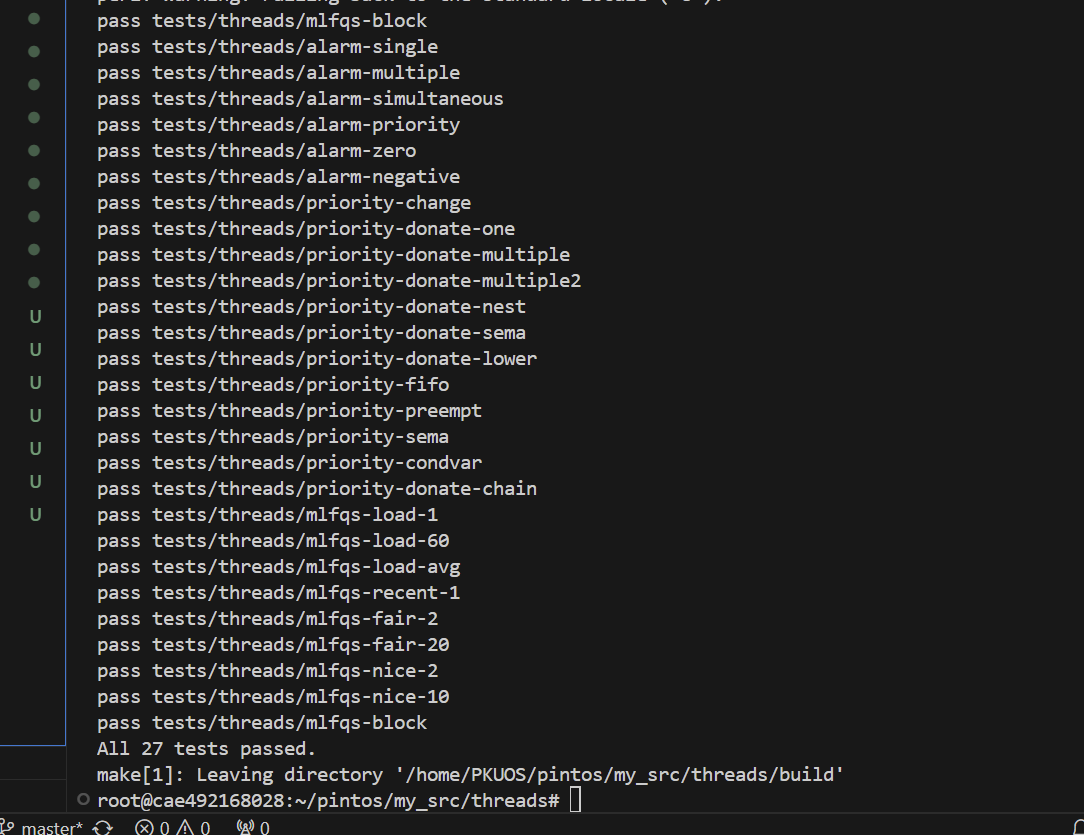
\includegraphics[width=10cm]{./img-project1/result.jpg}
		\caption{make check after processing project1}
		\label{fig:graph2}
	\end{figure}
	
	\subsection{实验过程}
	
	在实验中,完成实验的过程如上文所示:
	
	\setlength{\parindent}{2em}
	
	1. Mission-1: 重新实现timer-sleep()函数
	
	\setlength{\parindent}{4em}
	
	分析原本的timer\_sleep()函数的实现思路
	
	重新实现timer\_sleep()函数
	
	\setlength{\parindent}{2em}
	
	2. Mission-2: 重新实现timer-sleep()函数
	
	\setlength{\parindent}{4em}
	
	依次修改三个有关插入线程的函数,通过测试 \texttt{alarm\_priority}
	
	通过测试 \texttt{alarm-priority, priority-change, priority-fifo} 和 \texttt{priority-preempt}
	
	通过测试 \texttt{priority-priority-*}
	
	通过测试\texttt{priority-donate-multiple}和 \texttt{priority-donate-multiple2}
	
	通过测试\texttt{priority-donate-nest}
	
	通过测试\texttt{priority-donate-sema}
	
	通过测试\texttt{priority-donate-lower}(顺便通过了测试 \texttt{priority-sema} )
	
	通过测试\texttt{priority-condvar}(顺便通过了测试 \texttt{priority-donate-chain} )
	
	\setlength{\parindent}{2em}
	
	\subsection{实验分析}
	
	具体实验分析可以参考上文。
	
	通过 \texttt{diff -urNa ~/original-pintos/  ~/pintos/  >  project1.527.GuYiwei.patch} 之后,得到补丁文件,部分内容如下图所示:
	
	\begin{figure}[htbp]
		\centering
		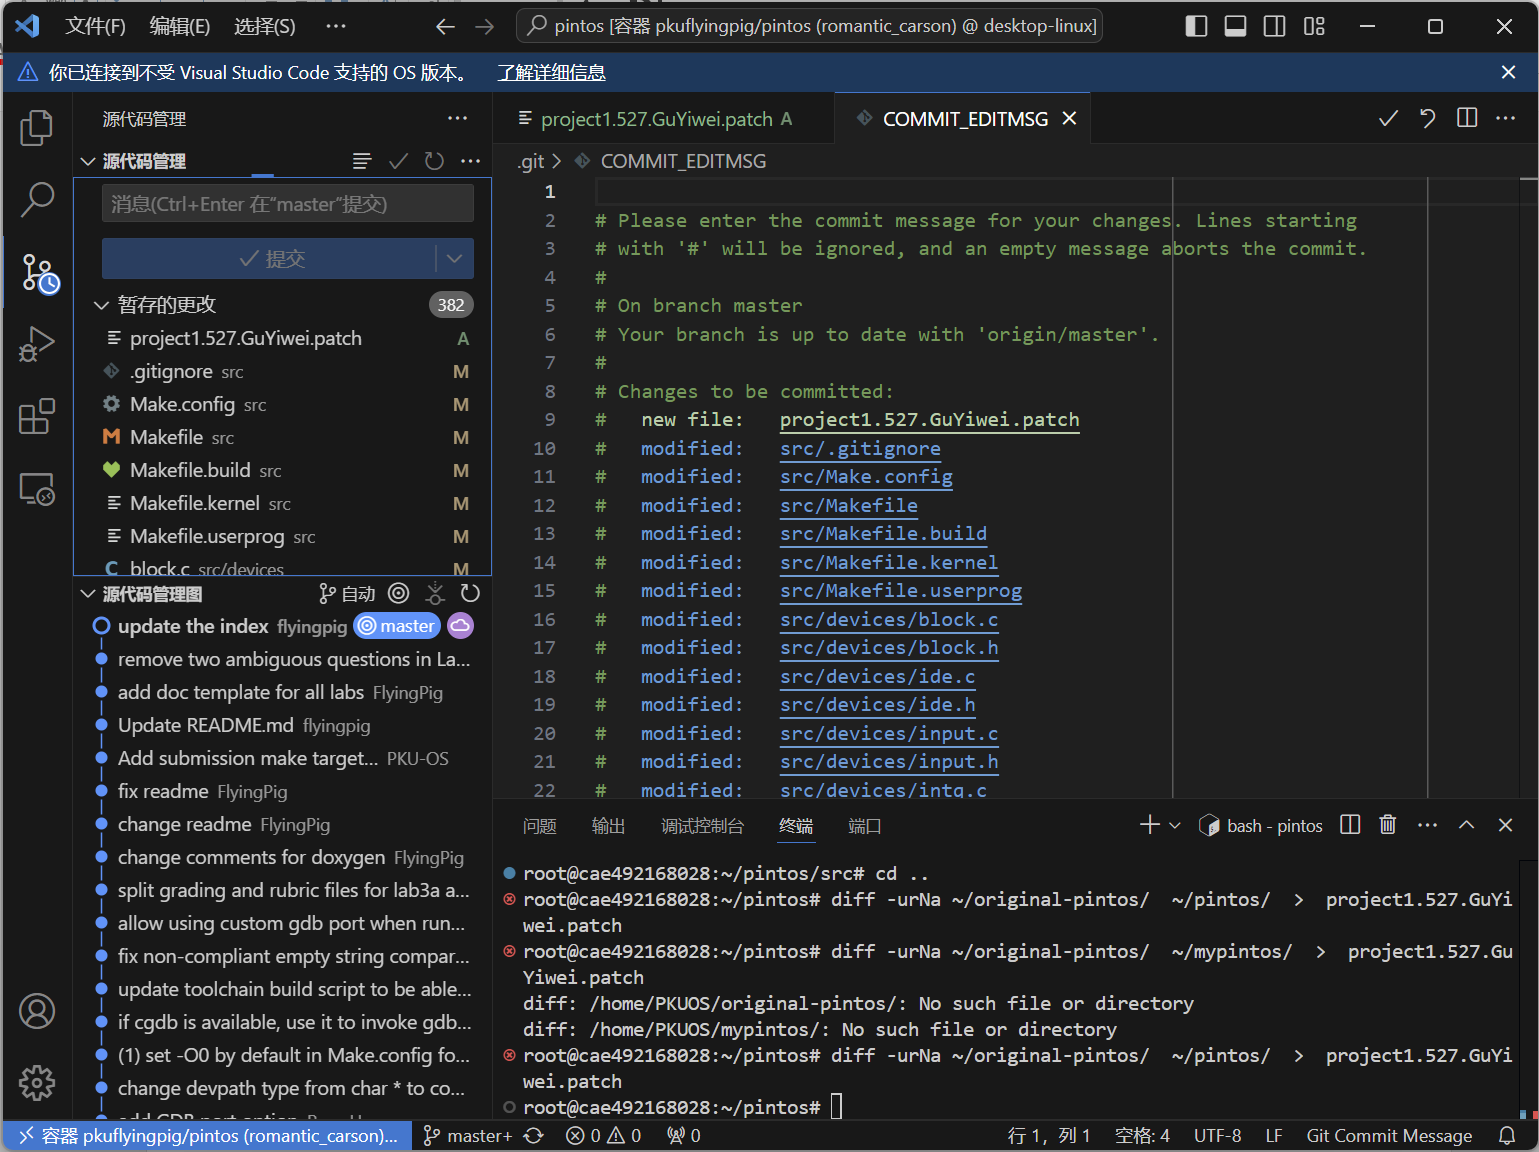
\includegraphics[width=13cm]{./img-project1/patch.jpg}
		\caption{make patch after finishing project1}
		\label{fig:graph3}
	\end{figure}
	
	\section{实验结果总结}
	
	在这次实验中,我对 \texttt{timer\_sleep()} 函数进行了重新设计,使其能够支持线程按设定的时间进行休眠,并在休眠期满后被重新激活。此外,我还引入了基于优先级的线程调度机制,确保线程能够依据其优先级获得相应的调度。
	
	通过这些实践活动,我不仅加深了对操作系统线程调度机制的理解,还对操作系统的整体实现有了更加深刻的洞察。
	
	\section{附录(源代码)}
	
	由于代码篇幅较长,我将修改好的代码放在了GitHub仓库;
	
	可以访问:\texttt{https://github.com/SoftGhostGU/OS/tree/main/OS\_project\_1}。
	
\end{document}